\documentclass[dvipsnames]{beamer}

\usepackage{amsmath,amssymb,bm}
\usetheme{sintef}

\usetikzlibrary{arrows,shapes,tikzmark,calc}

\usepackage{ctex}
\usepackage{fontspec}
\newCJKfontfamily\titlefont[
  BoldFont=LXGWZhenKaiGB-Regular.ttf,
  Path=fonts/
]{LXGWWenKai-Regular.ttf}
\usefonttheme[onlymath]{serif}

% fontspec resets \hbar at document start; restore the AMS glyph afterwards.
\AddToHook{begindocument/end}{\let\hbar\hslash}

% Reuse the template's restrained formula-annotation mechanism.
\newcommand{\highlight}[2]{\colorbox{#1!15}{#2}}
\newcommand{\physmark}[3]{%
  \tikzmarknode{#2}{\highlight{#1}{\color{black}$#3$}}%
}

\newcommand{\ii}{\mathrm{i}}
\newcommand{\Tr}{\operatorname{Tr}}
\newcommand{\papersource}[1]{%
  \par\vspace{0.2em}\hfill{\tiny\color{gray}#1}\par
}
\newcommand{\keypoint}[1]{%
  \begin{block}{核心结论}
    #1
  \end{block}
}



\title{{\fontsize{22}{25}\selectfont
  分子极化激元的\\线性响应与超快动力学}}
\subtitle{Linear Response and Ultrafast Dynamics of Molecular Polaritons}
\author{郭晋康}
\date{2026年9月8日}

\begin{document}

\maketitle

\section{分子极化激元与线性响应}
\begin{frame}{微观模型：分子 Hamiltonian 与腔场偶极耦合}
  \setlength{\abovedisplayskip}{0pt}
  \setlength{\belowdisplayskip}{0pt}
  \[
    H=H_0+V,
    \quad
    H_0=H_{\mathrm{ph}}+H_{\mathrm{mol}},
    \quad
    H_{\mathrm{ph}}=\hbar\omega_{\mathrm{ph}}a^\dagger a,
  \]

  \[
    V=-\physmark{Plum}{p4lambda}{\hbar\lambda}
    (a+a^\dagger)
    \physmark{Bittersweet}{p4mu}{\hat\mu},
    \quad
    \hat\mu=\sum_{i=1}^{N}\hat\mu_i(\bm q_i,\bm Q_i),
    \quad
    \hbar\lambda=
    \sqrt{\tfrac{\hbar\omega_{\mathrm{ph}}}{2\epsilon_0V}}.
  \]
  \begin{tikzpicture}[overlay,remember picture,>=stealth,
      nodes={align=center,inner ysep=1pt,font=\scriptsize},<-]
    \path (p4lambda.south) ++ (-1.5,-0.4em)
      node[anchor=north,color=Plum!85] (p4lambdatext)
      {\textsf{\footnotesize 真空腔场耦合强度}};
    \draw[color=Plum] (p4lambda.south) |- (p4lambdatext.north);
    \path (p4mu.south) ++ (1.5,-1em)
      node[anchor=north,color=Bittersweet!85] (p4mutext)
      {\textsf{\footnotesize 分子系综总偶极矩}};
    \draw[color=Bittersweet] (p4mu.south) |- (p4mutext.north);
  \end{tikzpicture}

  \[
    H_{\mathrm{mol}}
    =\sum_{i=1}^{N}
      \physmark{sintefgreen}{p3Hi}{H_i}
      \bigl(\physmark{OliveGreen}{p3qi}{\bm q_i},
      \physmark{sintefdarkgreen}{p3Qi}{\bm Q_i}\bigr)
    =\sum_y
      \physmark{sintefdarkgreen}{p3ey}{\hbar\Omega_y|y\rangle\langle y|}.
  \]
  \begin{tikzpicture}[overlay,remember picture,>=stealth,
      nodes={align=center,inner ysep=1pt,font=\scriptsize},<-]
    \path (p3qi.south) ++ (-0.55,-1.5em)
      node[anchor=north,color=OliveGreen!85] (p3qitext)
      {\textsf{\footnotesize 电子}};
    \draw[color=OliveGreen] (p3qi.south) |- (p3qitext.north);
    \path (p3Qi.south) ++ (0.55,-1.5em)
      node[anchor=north,color=sintefdarkgreen!85] (p3Qitext)
      {\textsf{\footnotesize 核}};
    \draw[color=sintefdarkgreen] (p3Qi.south) |- (p3Qitext.north);
    \path (p3ey.south) ++ (0.85,-1.5em)
      node[anchor=north,color=sintefdarkgreen!85] (p3eytext)
      {\textsf{\footnotesize 本征能量与多体本征态}};
    \draw[color=sintefdarkgreen] (p3ey.south) |- (p3eytext.north);
  \end{tikzpicture}
  \vspace{1.2em}

  {\centering\scriptsize
    电子结构、核振动、非谐性与多能级跃迁仍保留在
    $H_i(\bm q_i,\bm Q_i)$ 和 $\hat\mu_i$ 中。\par}
  \papersource{Yuen-Zhou \& Koner, JCP 160, 154107 (2024), Eqs.~(1)--(5).}
\end{frame}

\begin{frame}[c]{相同二能级分子的集体亮态与暗态}
  \small
  $N$ 个相同二能级分子、均匀单分子耦合 $g$、单激发子空间 定义亮态与暗态：

  \vspace{0.2em}
  {\centering\normalsize
    \(\displaystyle
      |B\rangle=\frac{1}{\sqrt N}\sum\nolimits_{j=1}^{N}|e_j\rangle,
    \qquad
      \langle D_\mu|B\rangle=0
    \)
    \par}

  \vspace{0.2em}
  {
    集体亮态是单激发在 $N$ 个分子之间的对称相干叠加；在相同二能级分子与旋波近似下

    ( Tavis--Cummings):\par}

  \vspace{1.5em}

  {\centering\small
    \(\displaystyle
      \begin{aligned}
        V_{\mathrm{RWA}}
          &=\hbar g\sum\nolimits_{j=1}^{N}
            \left(a^\dagger\sigma_j^-+a\sigma_j^+\right),
        \qquad
        B^\dagger
          =\frac{1}{\sqrt N}\sum\nolimits_{j=1}^{N}\sigma_j^+,
        \\ \\
        V_{\mathrm{RWA}}
          &=\hbar\physmark{Plum}{p5Gcoupling}{G}
            \left(a^\dagger B+aB^\dagger\right),
        \qquad
        \physmark{Plum}{p5G}{G}
          =\physmark{NavyBlue}{p5g}{g}
            \physmark{OliveGreen}{p5sqrtN}{\sqrt N}.
      \end{aligned}
    \)
    \par}
  \begin{tikzpicture}[overlay,remember picture,>=stealth,
      nodes={align=center,inner ysep=1pt},<-]
    \path (p5G.north) ++ (-1.25,-2.6em)
      node[anchor=east,color=Plum!85] (p5Gtext)
      {\textsf{\footnotesize 集体耦合}};
    \draw[color=Plum] (p5G.south) |- (p5Gtext.east);
    \path (p5g.north) ++ (0,-3.6em)
      node[anchor=south,color=NavyBlue!85] (p5gtext)
      {\textsf{\footnotesize 单分子耦合}};
    \draw[color=NavyBlue] (p5g.south) -- (p5gtext.north);
    \path (p5sqrtN.north) ++ (1.05,-2.6em)
      node[anchor=west,color=OliveGreen!85] (p5sqrtNtext)
      {\textsf{\footnotesize 集体相干增强}};
    \draw[color=OliveGreen]
      (p5sqrtN.south) |- (p5sqrtNtext.west);
  \end{tikzpicture}

  \vspace{2.0em}
\end{frame}

\begin{frame}[c]{腔光子与集体亮态杂化形成分子极化激元}
  \small
  集体亮态 $|B\rangle$与腔光子态构成基矢
  $|1_{\mathrm{cav}},\mathrm{GS}\rangle$、$|0_{\mathrm{cav}},B\rangle$。

  \vspace{0.8em}
  {\large
  \begin{equation*}
    H_{\mathrm{1exc}}=\hbar
    \begin{pmatrix}
      \physmark{Plum}{p6wc}{\omega_c} &
      \physmark{Bittersweet}{p6G}{G}\\[0.2em]
      G &
      \physmark{NavyBlue}{p6w0}{\omega_0}
    \end{pmatrix}.
  \end{equation*}}

  \begin{tikzpicture}[overlay,remember picture,>=stealth,
      nodes={align=center,inner ysep=1pt},<-]

    \path (p6wc.north) ++(-1.3,1.1em)
      node[anchor=south,color=Plum!85] (p6wctext)
      {\textsf{\footnotesize 单模腔频率}};
    \draw[color=Plum] (p6wc.north) |- (p6wctext.south);

    \path (p6w0.south) ++(1.4,-1.5em)
      node[anchor=north,color=NavyBlue!85] (p6w0text)
      {\textsf{\footnotesize 集体亮态频率}};
    \draw[color=NavyBlue] (p6w0.south) |- (p6w0text.north);

    \path (p6G.east) ++(1.4,1.1em)
      node[anchor=west,color=Bittersweet!85] (p6Gtext)
      {\textsf{\footnotesize 集体耦合}\\[-0.1em]
       \textsf{\footnotesize $G=g\sqrt{N}$}};
    \draw[color=Bittersweet] (p6G.north) |- (p6Gtext.west);

  \end{tikzpicture}

  \vspace{1.4em}

  {\large
  \begin{equation*}
    \omega_\pm=\frac{\omega_c+\omega_0}{2}
    \pm\sqrt{G^2+\frac{(\omega_c-\omega_0)^2}{4}}.
  \end{equation*}}

  \vspace{0.4em}

  {\footnotesize
    分子极化激元：腔光子模式与分子集体激发强耦合杂化的光--物质混合本征模（UP/LP）。\par}

\end{frame}

\begin{frame}[c]{分子极化与线性极化率}
  \small
  在线性响应近似下，只保留外场诱导极化的一阶项：

  {\centering\large
    \[
      \physmark{Plum}{p7dP}{\delta P^{(1)}(t)}
      =
      \int_{-\infty}^{t}
      \physmark{NavyBlue}{p7chi1}{\chi^{(1)}(t-t')}
      \physmark{Bittersweet}{p7Eweak}{E(t')}\,dt' .
    \]
    \par
  }

  \begin{tikzpicture}[
      overlay,
      remember picture,
      >=stealth,
      nodes={align=center,inner ysep=1pt},
      <-
    ]

    \path (p7dP.south) ++(-1.15,-0.75em)
      node[
        anchor=north,
        color=Plum!85
      ] (p7dPtext)
      {\textsf{\footnotesize 一阶诱导极化}};

    \draw[color=Plum]
      (p7dP.south) |- (p7dPtext.north);

    \path (p7chi1.south) ++(0,-0.75em)
      node[
        anchor=north,
        color=NavyBlue!85
      ] (p7chi1text)
      {\textsf{\footnotesize 线性极化响应}};

    \draw[color=NavyBlue]
      (p7chi1.south) |- (p7chi1text.north);

    \path (p7Eweak.south) ++(1.05,-0.75em)
      node[
        anchor=north,
        color=Bittersweet!85
      ] (p7Eweaktext)
      {\textsf{\footnotesize 弱外电场}};

    \draw[color=Bittersweet]
      (p7Eweak.south) |- (p7Eweaktext.north);

  \end{tikzpicture}

  \vspace{1.4em}

  \small
  $\chi^{(1)}(t-t')$ 描述分子受到时刻 $t'$ 的微弱电场扰动后，
  在时刻 $t$ 保留下来的偶极响应。

  {\centering\large
  \[
    \delta P^{(1)}(\omega)
    =
    \chi^{(1)}(\omega)E(\omega).
  \]
  \par}

  \vspace{0.5em}
  \small
  $\chi^{(1)}(\omega)$ 表征分子对频率为 $\omega$ 的弱外场产生的
  线性偶极响应强度与相位。

  \vspace{0.3em}
  {\color{gray}
    $\chi(\omega)$ 可由微观动力学或线性响应理论求得又或者线性吸收、色散或复折射率实验。
  }

\end{frame}


\section{\texorpdfstring{$N\to\infty$}{N to infinity} 极限下的线性光谱}
\begin{frame}{有效过程及初态条件}
  \small
  \begin{columns}[T,onlytextwidth]
    \begin{column}{0.49\textwidth}
      \vspace{2em}

      \hspace*{-0.30\linewidth}%
      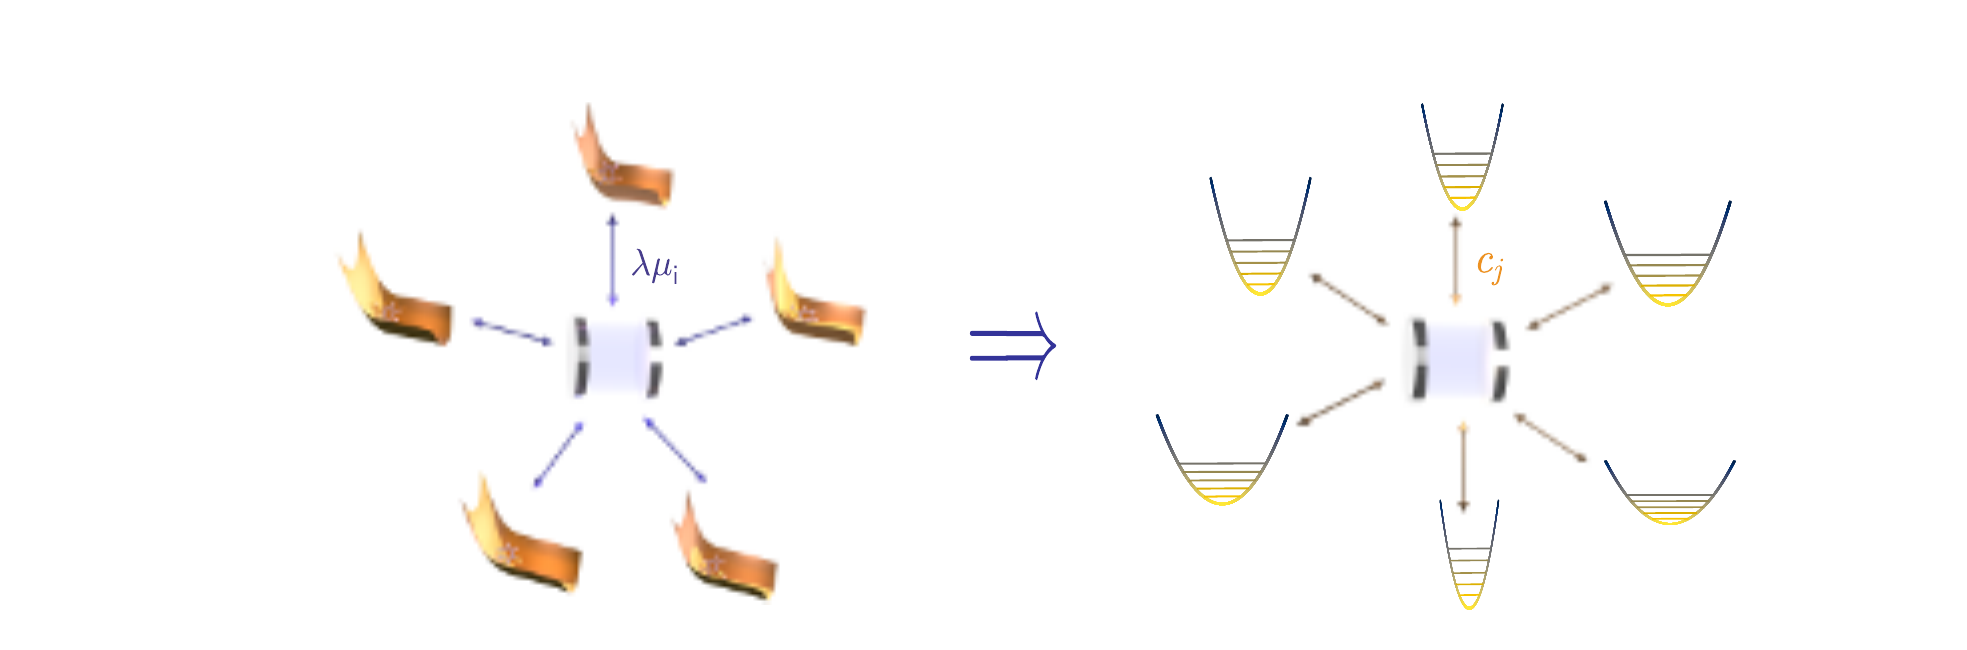
\includegraphics[width=1.5\linewidth,keepaspectratio]
        {figures/jcp_fig1_original.png}

    \end{column}
    \begin{column}{0.47\textwidth}
      \footnotesize

      将单模腔光子视为系统，分子系综视为环境。
      首先要求初态满足

      \[
        \rho(t_{\mathrm{in}})
        =
        \rho_{\mathrm{ph}}\otimes\rho_{\mathrm{mol}}
        =
        \rho_{\mathrm{ph}}\otimes
        \sum_y p_y|y\rangle\langle y|.
      \]

      {\color{gray}\hfill JCP Eq.~(6)}

      初始光与物质无关联；$\rho_{\mathrm{mol}}$ 是
      $H_{\mathrm{mol}}$ 的平稳态，不要求热平衡。

      \vspace{0.7em}

    \end{column}
  \end{columns}

  \papersource{Yuen-Zhou \& Koner,
  J. Chem. Phys. 160, 154107 (2024), Fig.~1.}
\end{frame}

\begin{frame}{分子系综作为腔光子的有效环境}

  \footnotesize
  \setlength{\abovedisplayskip}{4pt}
  \setlength{\belowdisplayskip}{4pt}

  \vspace*{0.4em}
  腔通过分子系综总偶极与分子环境耦合。
  {\fontsize{10.95}{13}\selectfont
  \[
    \begin{aligned}
      \hat\mu
        &=\sum_{i=1}^{N}\hat\mu_i,\\[0.3em]
      C_2(t)
        &=|\hbar\lambda|^2
          \langle\hat\mu(t)\hat\mu(0)\rangle\\
        &=|\hbar\lambda|^2\sum_i
          \langle\hat\mu_i(t)\hat\mu_i(0)\rangle.
    \end{aligned}
  \]}

  \vspace{0.6em}
  $C_2(t)$ 描述 $t=0$ 的偶极涨落经过时间 $t$ 后仍保留多少相关性。

  \vspace{0.8em}
  在 $N\to\infty$ 条件下，可用一个产生相同两时刻偶极关联的
  谐振子环境替代原复杂分子环境。
  {\fontsize{10.95}{13}\selectfont
  \[
    C_2^{\mathrm{eff}}(t)=C_2(t).
  \]}

  \papersource{JCP 160, 154107 (2024), Sec.~II, Eqs.~(13)--(14) 及 Eq.~(18) 。}

\end{frame}

\begin{frame}{谐振子环境的两时刻关联与有效谱密度}

  \footnotesize
  \setlength{\abovedisplayskip}{3pt}
  \setlength{\belowdisplayskip}{3pt}

  \vspace*{0.4em}
  等效谐振子环境由一组独立模式组成：
  {\fontsize{10.95}{13}\selectfont
  \[
    H_{\mathrm{mol}}^{\mathrm{eff}}
      =\sum\nolimits_j\hbar\omega_j b_j^\dagger b_j .
  \]}

  其谱密度定义为
  {\fontsize{10.95}{13}\selectfont
  \[
    J^{\mathrm{eff}}(\omega)
      \equiv\Theta(\omega)\pi\hbar
      \sum\nolimits_j|\bar c_j|^2\delta(\omega-\omega_j).
  \]}
  $J^{\mathrm{eff}}(\omega)$ 描述谐振子环境
  在不同频率处与腔模的耦合强度。

  \vspace{0.5em}
  对于线性谐振子环境，谱密度、模式布居和两时刻关联之间的关系是已知的。
  利用上一页的匹配条件 $C_2^{\mathrm{eff}}(t)=C_2(t)$，
  并结合正、负频率关系消去有效模式的布居信息，
  可得到 JCP Eq.~(18)：
  {\fontsize{10.95}{13}\selectfont
  \[
    J^{\mathrm{eff}}(\omega)
      =\frac{\ii\Theta(\omega)}{\hbar}
        \int_{-\infty}^{\infty}C_2(t)\sin(\omega t)\,dt.
  \]}

  因此真实分子的 $C_2(t)$ 已经足以确定
  等效谐振子环境的频率与耦合强度分布。

  \papersource{JCP 160, 154107 (2024), Eqs.~(8), (11), (13), (18).}

\end{frame}

\begin{frame}{有效谱密度由分子线性极化率给出}

  \scriptsize
  \setlength{\abovedisplayskip}{1pt}
  \setlength{\belowdisplayskip}{1pt}

  \vspace*{0.15em}
  {\fontsize{10}{12}\selectfont
  \[
    C_2(t)
    =\lim_{\gamma\to0^+}\sum\nolimits_{y,z}p_y
      |\hbar\lambda\langle z|\hat\mu|y\rangle|^2
      e^{-\ii(\omega_{zy}-\ii\gamma/2)t}.
  \]}
  将真实分子的两时刻偶极关联在 $H_{\mathrm{mol}}$ 本征态中展开：
  它是所有允许分子跃迁的叠加，
  每一项由跃迁频率、跃迁偶极和初态布居决定。

  \vspace{0.1em}
  将上述 $C_2(t)$ 代入上一页 Eq.~(18)，得到
  {\fontsize{10}{12}\selectfont
  \[
    J^{\mathrm{eff}}(\omega)
    =\Theta(\omega)\pi\hbar\sum\nolimits_{y,z}
      (p_y-p_z)|\lambda\langle z|\hat\mu|y\rangle|^2
      \delta(\omega_{zy}-\omega).
  \]}

  同一组分子跃迁也决定线性极化率。
  论文将其写成本征态谱表示（JCP Eq.~21b）：
  {\fontsize{10}{12}\selectfont
  \[
    \chi(\omega)
    =-\lim_{\gamma\to0^+}\sum\nolimits_{y,z}(p_y-p_z)
      \frac{|\lambda\langle z|\hat\mu|y\rangle|^2}
      {\omega-\omega_{zy}+\ii\gamma/2}.
  \]}

  $\operatorname{Im}\chi(\omega)$ 给出这组允许跃迁的吸收部分，
  因此论文 Eq.~(20) 得到
  {\fontsize{10}{12}\selectfont
  \[
    J^{\mathrm{eff}}(\omega)
    =\Theta(\omega)\hbar\,\operatorname{Im}\chi(\omega).
  \]}
  等效谐振子环境在各频率处需要多强地耦合，
  恰好由真实分子在这些频率处的吸收响应决定。

  \papersource{JCP 160, 154107 (2024), Eqs.~(18)--(21).}

\end{frame}

\begin{frame}{$N\to\infty$ 下：弱 probe 读取微腔线性光谱}

  \label{frame:cavity-response}

  \footnotesize
  \setlength{\abovedisplayskip}{2pt}
  \setlength{\belowdisplayskip}{2pt}

  $\omega_{\mathrm{ph}}$ 是固定的裸腔共振频率，
  裸分子系综对 probe 的线性响应由 $\chi(\omega)$ 给出。
  标准输入--输出理论将腔内线性响应转换为透射、反射和吸收光谱：

  \[
    T(\omega)
    =
    \frac{\kappa_L\kappa_R}
    {\left|
      \physmark{Plum}{p14det}{\omega-\omega_{\mathrm{ph}}}
      +
      \physmark{Bittersweet}{p14loss}{\ii\kappa/2}
      +
      \physmark{NavyBlue}{p14chi}{\chi(\omega)}
    \right|^2}.
  \]

  \begin{tikzpicture}[
      overlay,
      remember picture,
      >=stealth,
      nodes={align=center,inner ysep=1pt},
      <-
    ]

    \path (p14det.south) ++ (-1.4,-1.0em)
      node[anchor=north,color=Plum!85] (p14dettext)
      {\textsf{\footnotesize probe--裸腔失谐}};
    \draw[color=Plum]
      (p14det.south) |- (p14dettext.north east);

    \path (p14loss.south) ++ (0,-1.0em)
      node[anchor=north,color=Bittersweet!85] (p14losstext)
      {\textsf{\footnotesize 腔光子损耗}};
    \draw[color=Bittersweet]
      (p14loss.south) -- (p14losstext.north);

    \path (p14chi.south) ++ (1.4,-1.0em)
      node[anchor=north,color=NavyBlue!85] (p14chitext)
      {\textsf{\footnotesize 分子线性响应}};
    \draw[color=NavyBlue]
      (p14chi.south) |- (p14chitext.north west);

  \end{tikzpicture}

  \vspace{2.2em}

  \[
    A(\omega)
    =
    \frac{2\kappa_L\operatorname{Im}\chi(\omega)}
    {|\omega-\omega_{\mathrm{ph}}+\ii\kappa/2+\chi(\omega)|^2},
    \qquad
    R(\omega)=1-T(\omega)-A(\omega).
  \]

\vspace{1em}
  {\scriptsize\color{gray}
    线性响应表示 probe 足够弱，只保留外场诱导响应的一阶项。\\[-0.1em]

    左侧入射，$\kappa=\kappa_L+\kappa_R$；
    旋波近似、Markov 输入--输出理论；详细推导见末页理论补充。\par}

  \papersource{JCP 160, 154107 (2024), Table~I, Eqs.~(27), (34a,b).}

\end{frame}
\begin{frame}{二能级分子线性响应}
  \fontsize{7.3}{8.4}\selectfont
  \setlength{\abovedisplayskip}{1.5pt}
  \setlength{\belowdisplayskip}{1.5pt}
  \setlength{\abovedisplayshortskip}{0pt}
  \setlength{\belowdisplayshortskip}{0pt}
  \begin{columns}[T,onlytextwidth]
    \begin{column}{0.51\textwidth}
      \[
        \begin{aligned}
        \chi_{\mathrm{2LS}}(\omega)
        &=-\frac{N|g|^2}
        {\omega-\omega_{\mathrm{exc}}+i\gamma/2}
        =-\frac{G^2}
        {\omega-\omega_{\mathrm{exc}}+i\gamma/2},\\[-0.1em]
        &\hspace{7em}G^2=N|g|^2.
        \end{aligned}
      \]
      \vspace{0.25em}
      零失谐时
      \[
        \omega_{\mathrm{ph}}=\omega_{\mathrm{exc}}\equiv\omega_0.
      \]
      {\scriptsize\color{gray}
        为说明双峰位置，先忽略损耗。\par}

      \[
        (\omega-\omega_0)^2-G^2=0,
        \qquad
        \boxed{\omega_{\mathrm{LP/UP}}=\omega_0\mp G}.
      \]
      \vspace{1.5em}
      {\scriptsize\color{gray}
        加入损耗后，复频率满足
        $(\omega-\omega_{\mathrm{ph}}+i\kappa/2)
        (\omega-\omega_{\mathrm{exc}}+i\gamma/2)-G^2=0$；
        其实部给出共振尺度，虚部给出衰减/线宽。\par}
    \end{column}
    \begin{column}{0.47\textwidth}
      {\centering
        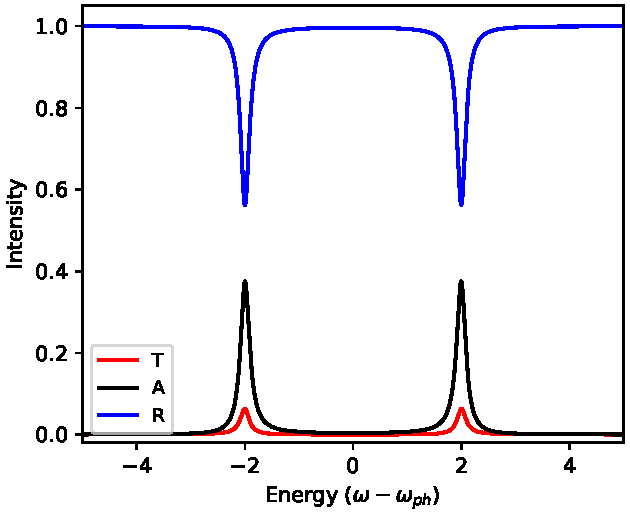
\includegraphics[width=\linewidth,height=0.60\textheight,keepaspectratio]
          {figures/linear_fig3a_reproduction.pdf}\\[-0.2em]
        $\omega-\omega_{\mathrm{ph}}$ {\scriptsize probe 相对于腔共振的频率失谐\par}
        \vspace{0.25em}}
    \end{column}
  \end{columns}
  \vspace{2.5em}
  {\centering\textbf{强耦合形成 LP/UP 两个本征模；
    弱 probe 扫描其本征频率，并在 $T/R/A$ 中读出双峰/双谷共振结构。}\par}
  \papersource{JCP 160, 154107 (2024), Eqs.~(37), (38), (40), Fig.~3(a).}
\end{frame}

\begin{frame}{二能级极化激元的布居与无序效应}
  \fontsize{7}{7.9}\selectfont
  \setlength{\abovedisplayskip}{1pt}
  \setlength{\belowdisplayskip}{1pt}
  \setlength{\abovedisplayshortskip}{0pt}
  \setlength{\belowdisplayshortskip}{0pt}
  \vspace{0.2em}
  \begin{columns}[T,onlytextwidth]
    \begin{column}{0.49\textwidth}
      {\centering
        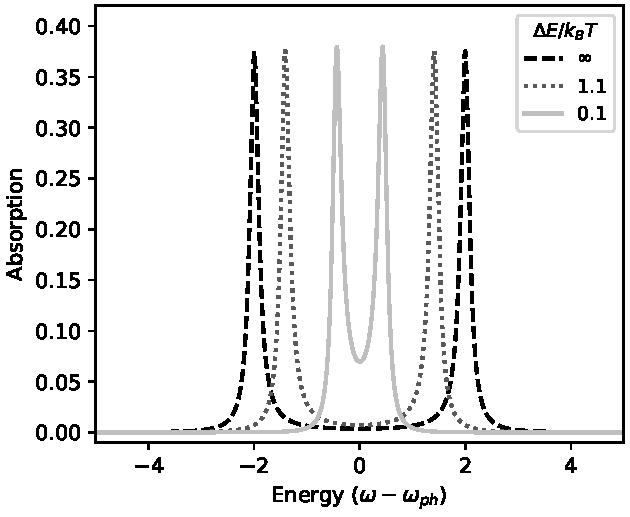
\includegraphics[width=\linewidth,height=0.52\textheight,keepaspectratio]
          {figures/linear_fig3b_reproduction.pdf}\par}
      {\scriptsize\color{gray}$G=2$，$\kappa=0.1$，$\gamma=0.3$，
        $\Delta E/(k_BT)=\infty,\,1.1,\,0.1$。\par}
      \[
        \physmark{NavyBlue}{p17pop}{
          p_g-p_e
          =
          \tanh\!\left(\frac{\Delta E}{2k_BT}\right)},
        \quad
        \chi_{\mathrm{2LS}}\propto
        \physmark{Plum}{p17split}{p_g-p_e}.
      \]
      布居差减小 $\rightarrow$ 分子线性响应减弱
      $\rightarrow$ Rabi 劈裂收缩。
    \end{column}
    \begin{column}{0.49\textwidth}
      {\centering
        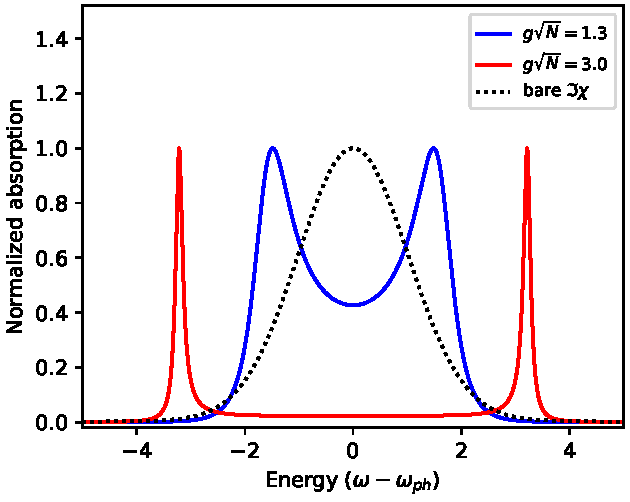
\includegraphics[width=\linewidth,height=0.52\textheight,keepaspectratio]
          {figures/linear_fig4c_reproduction.pdf}\par}
      {\scriptsize\color{gray}$\sigma=1$，$\kappa=\gamma=0.1$，
        比较 $G=1.3$ 与 $3.0$。\par}
      \[
        \physmark{NavyBlue}{p17sigma}{
          \omega_{\mathrm{exc}}
          \sim
          \mathcal N(\bar\omega,\sigma^2)},
        \quad
        \physmark{Plum}{p17ratio}{G/\sigma\uparrow}.
      \]
      当集体耦合超过非均匀展宽尺度时，
      极化激元线宽更多由均匀线宽与腔损耗决定。
    \end{column}
  \end{columns}
  \vspace{1.5em}
  {\centering\textbf{改变的都是分子侧 $\chi(\omega)$；
    上一页 $T/R/A$ 的通用形式保持不变。}\par}
  \papersource{JCP 160, 154107 (2024), Eqs.~(37), (41), (42), Figs.~3(b), 4(c).}
\end{frame}


\section{从稳态响应到超快非平衡动力学}
\begin{frame}{从稳态线性响应到超快 pump--probe}

  \footnotesize
  \setlength{\abovedisplayskip}{1pt}
  \setlength{\belowdisplayskip}{1pt}

  {\centering
    $\text{weak probe}\;\longrightarrow\;\chi(\omega)
      \;\longrightarrow\;T(\omega),R(\omega),A(\omega).$\par}
  {\centering\fontsize{6.5}{7.6}\selectfont\color{gray}
    平稳腔--分子体系可由固定的线性响应 $\chi(\omega)$ 描述。\par}

  \vspace{0.1em}

  \begin{columns}[T,onlytextwidth]
    \begin{column}{0.44\textwidth}
      {\centering
        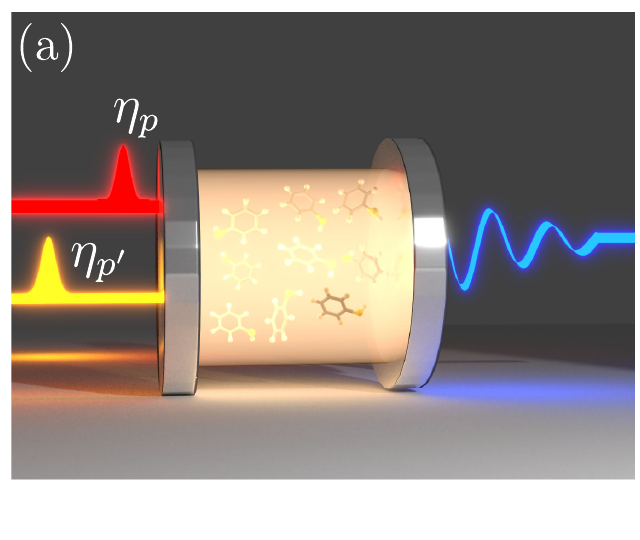
\includegraphics[width=\linewidth,height=0.55\textheight,keepaspectratio]
          {figures/prl_fig1a_cavity.png}\par}
      {\centering\fontsize{6.5}{7.6}\selectfont\color{gray}
        实验体系：分子系综位于光腔中，
        由 pump 和 probe 两束输入脉冲驱动。\par}
    \end{column}
    \begin{column}{0.54\textwidth}
      {\centering
        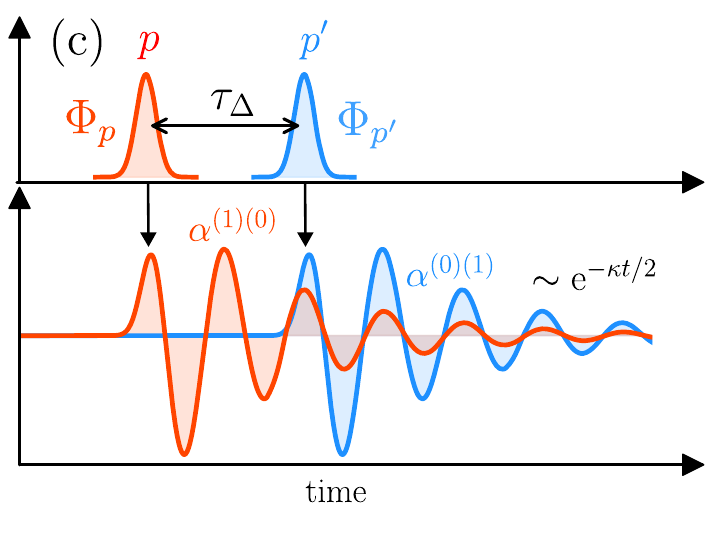
\includegraphics[width=\linewidth,height=0.55\textheight,keepaspectratio]
          {figures/prl_fig1c_pulse.png}\par}
      {\centering\fontsize{6.5}{7.6}\selectfont\color{gray}
        时间结构：$\tau_\Delta=\tau_{p'}-\tau_p$。由于腔内场具有有限寿命，某些微扰作用次序中 probe 场甚至可以先于 pump 场作用于分子体系。\par}
    \end{column}
  \end{columns}

  \vspace{0.8em}

  {\centering
    $\text{长延迟}\quad\Longrightarrow\quad
      \text{体系已接近稳/准稳状态，可近似使用 }\chi(\omega).$\\[0.2em]
    $\text{超短延迟？}$\\[0.2em]
    \par}

  \papersource{Reitz, Koner \& Yuen-Zhou,
    PRL 134, 193803 (2025), Fig.~1(a,c).}

\end{frame}
\begin{frame}{$N\to\infty$ 极限：腔场与单分子态自洽反馈}

  \footnotesize
  \setlength{\abovedisplayskip}{2pt}
  \setlength{\belowdisplayskip}{2pt}

  \[
    \begin{aligned}
      H_{\mathrm{MF}}(t)
        &=H_0+E_0[\alpha(t)+\alpha^*(t)]\hat\mu,\\[-1.5pt]
        \\
      \dot\rho
        &=-\ii[H_{\mathrm{MF}}(t),\rho]+\mathcal D[\rho].
    \end{aligned}
  \]

  \vspace{4em}

  \[
    \begin{aligned}
      \dot\alpha
        &=\physmark{Plum}{mfFree}{-\left(\tfrac{\kappa}{2}+\ii\omega_c\right)\alpha}
          \physmark{NavyBlue}{mfFeedback}{-\ii NE_0P}
          \physmark{OliveGreen}{mfInput}{-\eta f(t)e^{-\ii\omega_l t}},\qquad P&=\Tr[\hat\mu\rho].
    \end{aligned}
  \]
  \begin{tikzpicture}[overlay,remember picture,>=stealth,
      nodes={align=center,inner sep=1pt,font=\scriptsize},<-]
    \path (mfFree.north) ++(-1.5,1.0em)
      node[anchor=south,color=Plum] (mfFreeText)
      {腔模自由演化 + 振幅损耗};
    \draw[Plum] (mfFree.north) |- (mfFreeText.south);
    \path (mfFeedback.north) ++(0,1.0em)
      node[anchor=south,color=NavyBlue] (mfFeedbackText)
      {分子系综极化反馈};
    \draw[NavyBlue] (mfFeedback.north) -- (mfFeedbackText.south);
    \path (mfInput.north) ++(0.7,1.0em)
      node[anchor=south,color=OliveGreen] (mfInputText)
      {外部输入场驱动};
    \draw[OliveGreen] (mfInput.north) |- (mfInputText.south);
  \end{tikzpicture}

  \vspace{1em}
  {\centering
    \begin{tikzpicture}[>=stealth,thick,
        every node/.style={align=center,inner sep=3pt,font=\scriptsize}]
      \node[draw=Plum] (a) at (0,0)
        {$\alpha=\langle\hat a\rangle$\\腔内平均场};
      \node[draw] (h) at (3,0) {$H_{\mathrm{MF}}$\\驱动单分子};
      \node[draw] (r) at (6,0) {$\rho$\\分子量子态};
      \node[draw=NavyBlue] (p) at (9,0) {$P$\\单分子平均偶极};
      \draw[->] (a) -- (h);
      \draw[->] (h) -- (r);
      \draw[->] (r) -- (p);
      \draw[->,NavyBlue] (p.south) -- (9,-0.7)
        -- (0,-0.7) -- (a.south);
      \node[fill=white,text=NavyBlue] at (4.5,-0.7)
        {系综反馈：$NP$};
    \end{tikzpicture}\par}

  \papersource{Reitz, Koner \& Yuen-Zhou, PRL 134, 193803 (2025), Eqs.~(2)--(3).}

\end{frame}
\begin{frame}{腔内场与分子态的微扰展开}

  \footnotesize
  \setlength{\abovedisplayskip}{1pt}
  \setlength{\belowdisplayskip}{1pt}

  \[
    \alpha(t)=\sum_n\eta^n\alpha^{(n)}(t),
    \qquad
    \rho(t)=\sum_n\eta^n\rho^{(n)}(t).
  \]

  \vspace{0.3em}

  \begin{columns}[c,onlytextwidth]
    \begin{column}{0.48\textwidth}
      {\centering
        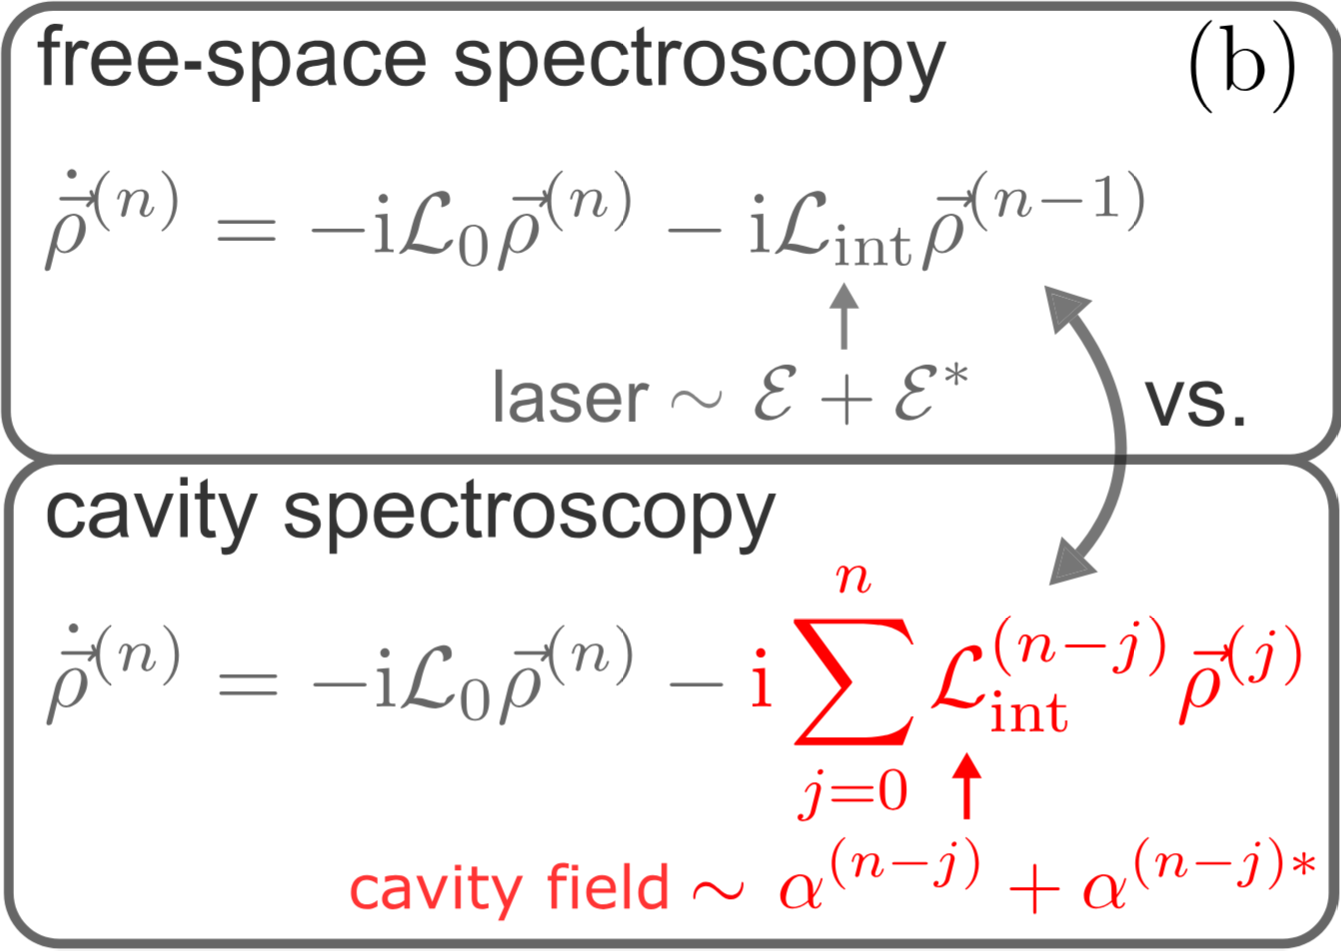
\includegraphics[width=\linewidth,keepaspectratio]{fig/fig1b.png}\par}
    \end{column}
    \begin{column}{0.50\textwidth}
      \scriptsize
      \[
        \dot\alpha^{(n)}
        =-\left(\tfrac{\kappa}{2}+\ii\omega_c\right)\alpha^{(n)}
        -\ii NE_0P^{(n)}
        -\physmark{OliveGreen}{ordDrive}{\delta_{n1}}
          f(t)e^{-\ii\omega_l t}.
      \]
      \begin{tikzpicture}[overlay,remember picture,>=stealth,
          nodes={align=center,inner sep=1pt,font=\scriptsize},<-]
        \path (ordDrive.south) ++(0.9,3.5em)
          node[anchor=north,color=OliveGreen,text width=3.0cm] (ordDriveText)
          {外部输入只驱动一阶};
        \draw[OliveGreen] (ordDrive.north) |- (ordDriveText.south);
      \end{tikzpicture}

      \vspace{3.5em}
      $n>1$ 的腔场由分子极化反馈产生。 

      自由空间：分子始终由给定的一阶激光场驱动；\\
      腔内：分子极化会产生新的高阶腔场。
  

    \end{column}
  \end{columns}

  \vspace{0.3em}

  \papersource{ PRL Fig.~1(b), p.~193803-2; Eqs.~(4)--(5).}
\end{frame}
\begin{frame}{腔反馈产生额外高阶演化路径}

  \footnotesize
  \setlength{\abovedisplayskip}{1pt}
  \setlength{\belowdisplayskip}{1pt}

  \[
    \physmark{NavyBlue}{p20tgt}{\dot{\vec\rho}^{(n)}}
    =\physmark{NavyBlue}{p20free}{-\ii\mathcal L_0\vec\rho^{(n)}}
    -\ii E_0\sum_{j=0}^{n}
    \physmark{Plum}{p20field}{
      \left[\alpha^{(n-j)}+\alpha^{(n-j)*}\right]}
    \mathcal L_\mu
    \physmark{Bittersweet}{p20rho}{\vec\rho^{(j)}}.
  \]
  \begin{tikzpicture}[overlay,remember picture,>=stealth,
      nodes={align=center,inner sep=1pt,font=\scriptsize},<-]
    \path (p20tgt.south) ++(-1.7,-1.1em)
      node[anchor=north,color=NavyBlue,text width=2.9cm] (p20tgtText)
      {目标：第 $n$ 阶分子响应};
    \draw[NavyBlue] (p20tgt.south) |- (p20tgtText.north);
    \path (p20free.south) ++(-0.3,-1.1em)
      node[anchor=north,color=NavyBlue!70!black,text width=2.6cm] (p20freeText)
      {自由演化，不产生新分支};
    \draw[NavyBlue!70!black] (p20free.south) -- (p20freeText.north);
    \path (p20field.south) ++(1.5,-1.1em)
      node[anchor=north,color=Plum,text width=2.2cm] (p20fieldText)
      {第 $n-j$ 阶腔场};
    \draw[Plum] (p20field.south) |- (p20fieldText.north);
    \path (p20rho.south) ++(2.6,-1.1em)
      node[anchor=north,color=Bittersweet,text width=2.6cm] (p20rhoText)
      {已有第 $j$ 阶分子响应};
    \draw[Bittersweet] (p20rho.south) |- (p20rhoText.north);
  \end{tikzpicture}
  \vspace{1.4em}

  \begin{columns}[c,onlytextwidth]
    \begin{column}{0.46\textwidth}
      {\centering
        \includegraphics[page=3,trim=321bp 565bp 57bp 47bp,clip,
          height=0.62\textheight,keepaspectratio]
          {../ref/Reitz 等 - 2025 - Nonlinear Semiclassical Spectroscopy of Ultrafast Molecular Polariton Dynamics.pdf}\par}
    \end{column}
    \begin{column}{0.52\textwidth}
      \scriptsize
      以二阶响应为例：
      \[
        \begin{aligned}
        \dot\rho^{(2)}
        &=-\ii\mathcal L_0\rho^{(2)}
          -\ii E_0\Big[
            (\alpha^{(1)}+\alpha^{(1)*})\mathcal L_\mu\rho^{(1)}\\
        &\qquad\quad
            +(\alpha^{(2)}+\alpha^{(2)*})\mathcal L_\mu\rho^{(0)}
          \Big].
        \end{aligned}
      \]
      {\color{gray}无外场时 $\alpha^{(0)}=0$。\par}
      \vspace{0.1em}
      {\centering\textcolor{orange!80!black}{%
        $\rho^{(0)}\xrightarrow{\alpha^{(1)}}
          \rho^{(1)}\xrightarrow{\alpha^{(1)}}\rho^{(2)}$}\par}
      \textcolor{orange!80!black}{连续两次一阶作用：自由空间已有的路径。}
      \par\vspace{0.1em}
      {\centering$\rho^{(0)}\xrightarrow{\alpha^{(2)}}\rho^{(2)}$\par}
      $\alpha^{(2)}$ 由分子极化反馈产生。
      \par\vspace{0.1em}
    \end{column}
  \end{columns}

  \papersource{Reitz, Koner \& Yuen-Zhou, PRL 134, 193803 (2025), Eq.~(5b), Fig.~2.}

\end{frame}


\section{泵浦--探测与超快非线性响应}
\begin{frame}{Pump--probe：双场展开与最低三阶响应}

  \footnotesize
  \setlength{\abovedisplayskip}{1.5pt}
  \setlength{\belowdisplayskip}{1.5pt}

  \begin{columns}[c,onlytextwidth]
    \begin{column}{0.62\textwidth}
      \[
        \alpha(t)=\sum_{n,m}\eta_p^n\eta_{p'}^m
          \alpha^{(n)(m)}(t),
        \qquad
        \rho(t)=\sum_{n,m}\eta_p^n\eta_{p'}^m
          \rho^{(n)(m)}(t).
      \]
      {\centering
        $(n,m)=(\text{pump 阶数},\,\text{probe 阶数})$。\par}
    \end{column}
    \begin{column}{0.36\textwidth}
      {\centering
        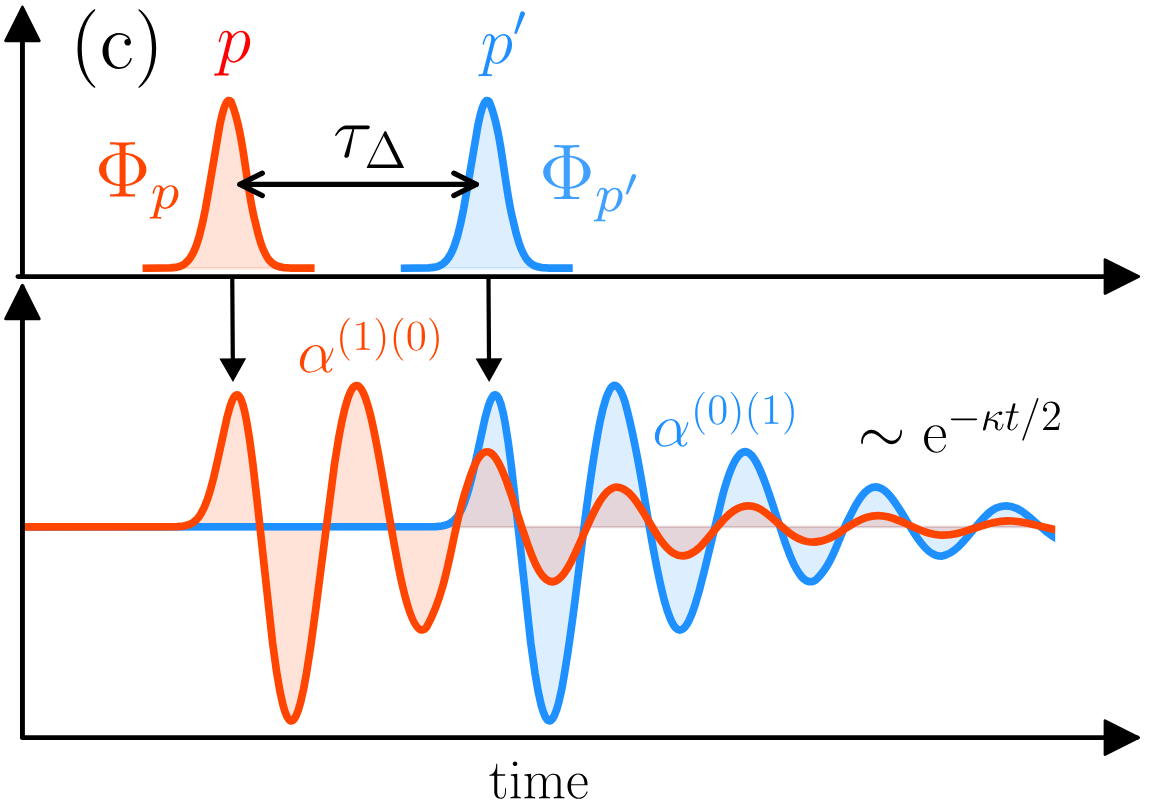
\includegraphics[width=0.76\linewidth,keepaspectratio]{../ref/fig1c.png}\par}
      {\centering\tiny\color{gray}
        $\tau_\Delta=\tau_{p'}-\tau_p$：pump 先作用，probe 延迟读取。\par}
    \end{column}
  \end{columns}

  \vspace{0.1em}

  {\centering\small
    相同二能级分子系综 + 单模腔
    $\xrightarrow{\;G=g\sqrt N\;}$ LP/UP。\par}
  {\centering\tiny\color{gray}
    pump 使体系偏离平衡，probe 延迟读取瞬态响应。\par}

  \vspace{0.15em}

  \begin{center}
  \begin{tikzpicture}[>=stealth,
      every node/.style={inner sep=2pt}]
    \node (r0) {$\rho^{(0)}$};
    \node (r1) at (3.1,0) {$\rho^{(1)(0)}$};
    \node (r2) at (6.2,0) {$\rho^{(2)(0)}$};
    \node (r3) at (9.3,0) {$\rho^{(2)(1)}$};
    \draw[->] (r0) -- node[above,font=\scriptsize]{\textcolor{Plum}{$p$}}
      node[below,font=\scriptsize]{相干} (r1);
    \draw[->] (r1) -- node[above,font=\scriptsize]{\textcolor{Plum}{$p$}}
      node[below,font=\scriptsize]{布居} (r2);
    \draw[->] (r2) -- node[above,font=\scriptsize]{\textcolor{NavyBlue}{$p'$}}
      node[below,font=\scriptsize]{读取} (r3);
    \draw[rounded corners=3pt,thin,black!50]
      ([xshift=-8pt,yshift=-5pt]current bounding box.south west)
      rectangle
      ([xshift=8pt,yshift=5pt]current bounding box.north east);
  \end{tikzpicture}
  \end{center}

  \vspace{0.2em}

  {\centering
    $p^2p'\ \Longrightarrow\ \alpha^{(2)(1)}$，\qquad
    这是二能级示例中的最低三阶 pump--probe 响应。\par}

  \papersource{Reitz, Koner \& Yuen-Zhou, PRL 134, 193803 (2025), Eq.~(6), Fig.~1(c).}

\end{frame}

\begin{frame}{差分透射谱}

  \footnotesize
  \setlength{\abovedisplayskip}{2pt}
  \setlength{\belowdisplayskip}{2pt}

  \begin{columns}[c,onlytextwidth]
    \begin{column}{0.48\textwidth}
      {\centering\fboxsep=5pt\fboxrule=0.4pt
      \fbox{\begin{minipage}{0.92\linewidth}
        {\centering\textbf{pump off}\par}
        \[
          \text{弱 probe}
          \rightarrow\alpha^{(0)(1)}(\omega)
          \rightarrow T_{\rm off}(\omega)
        \]
        {\centering\scriptsize
          线性基准：对应第一篇中的弱探测线性透射。\par}
      \end{minipage}}\par}
    \end{column}
    \begin{column}{0.48\textwidth}
      {\centering\fboxsep=5pt\fboxrule=0.4pt
      \fbox{\begin{minipage}{0.92\linewidth}
        {\centering\textbf{pump on}\par}
        \[
          \text{pump + probe}
          \rightarrow\alpha(\omega,\tau_\Delta)
          \rightarrow T_{\rm on}(\omega,\tau_\Delta)
        \]
        {\centering\scriptsize
          pump 改变体系后得到的瞬态探测透射。\par}
      \end{minipage}}\par}
    \end{column}
  \end{columns}

  \vspace{0.3em}

  \[
    T_{p'}(\omega)
    =\left|
      \frac{(\kappa/2)\,\alpha(\omega)}{\eta_{p'}f_{p'}(\omega)}
    \right|^2
    \qquad
    \Delta T(\omega,\tau_\Delta)
    =T_{\rm on}-T_{\rm off}
  \]
  {\centering\scriptsize\color{gray}
    二者都通过同一标准输入--输出关系由腔内场得到；
    区别只在于 pump on/off 时的腔内场不同。\par}

  \vspace{0.2em}

  {\centering\scriptsize
    $\Delta T>0$：透射增强；\qquad $\Delta T<0$：透射减弱。\par
    因此差分透射测量的是 pump 对原线性 probe 光谱的改变量。\par}

  \vspace{0.3em}

  \[
    \physmark{OliveGreen}{dtResult}{\Delta T^{(3)}(\omega)}
    \propto2\operatorname{Re}\!\left[
      \physmark{NavyBlue}{dtLO}{\alpha^{(0)(1)*}(\omega)}
      \physmark{Plum}{dtNL}{\alpha^{(2)(1)}(\omega)}
    \right].
  \]
  {\centering\scriptsize
    由于探测器测量强度 $T\propto|\alpha|^2$，
    线性 probe 场与三阶场的交叉项给出最低阶差分透射信号。\par}
  {\centering\tiny\color{gray}
    $\alpha^{(0)(1)}$：线性 probe 基准场；\quad
    $\alpha^{(2)(1)}$：pump 诱导的三阶场。\par}

  \papersource{PRL Eqs.~(7)--(8); SM Eqs.~(S.11)--(S.14).}

\end{frame}

\begin{frame}{Fig.~3：差分透射读取相干与布居的时间尺度}

  \footnotesize

  \begin{columns}[c,onlytextwidth]
    \begin{column}{0.61\textwidth}
      {\centering
        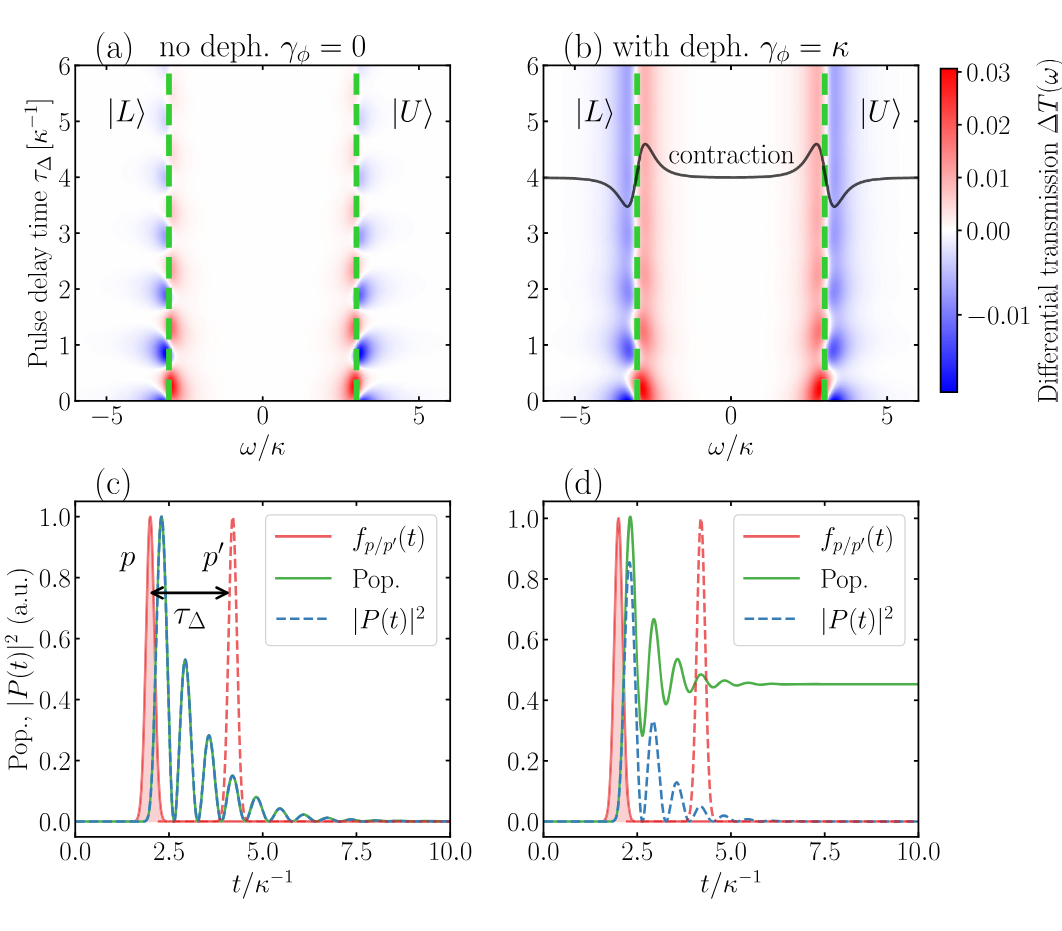
\includegraphics[width=0.85\linewidth,keepaspectratio]{../ref/fig3.png}\par}
    \end{column}
    \begin{column}{0.37\textwidth}
      {\scriptsize\color{gray}
        红：$\Delta T>0$，
        \\
        蓝：$\Delta T<0$；
        \\
        绿虚线：LP/UP 共振位置。\par}

      \vspace{0.6em}
      \textbf{(c)$\rightarrow$(a)，$\gamma_\phi=0$}\par
      {\scriptsize
        相干与布居振荡导致 UP--LP 相位拍频，
        因此 $\Delta T$ 随延迟出现红蓝交替条纹。\par}

      \vspace{0.6em}
      \textbf{(d)$\rightarrow$(b)，$\gamma_\phi=\kappa$}\par
      {\scriptsize
        退相使相干迅速衰减，但布居仍可保留，
        因此时间条纹消失，而长延迟下仍可见谱修正与劈裂收缩。\par}

    \end{column}
  \end{columns}

  \papersource{Original PRL Fig.~3(a--d), p.~193803-4; SM Eq.~(S.14), Fig.~S1.}

\end{frame}


\begin{frame}{总结：从线性响应到超快非平衡动力学}

  \small
  \setlength{\abovedisplayskip}{2pt}
  \setlength{\belowdisplayskip}{2pt}

  {\scriptsize\color{gray}JCP 2024\par}
  \[
    \text{强耦合 cavity--molecule system}
    \longrightarrow\chi(\omega)
    \longrightarrow T(\omega),\,R(\omega),\,A(\omega)
  \]
  {\centering\scriptsize
    弱 probe 读取已形成的 LP/UP 线性共振。\par}

  \vspace{0.3em}
  \[
    \text{pump 将体系推离平衡}
    \quad\Longrightarrow\quad
    \rho(t)\ \longleftrightarrow\ \alpha(t)
  \]
  {\centering\scriptsize
    分子态与腔场必须自洽实时演化，$P(t)=\Tr[\hat\mu\rho(t)]$。\par}

  \vspace{0.3em}
  {\scriptsize\color{gray}PRL 2025\par}
  \[
    p^2p'
    \longrightarrow\alpha^{(2)(1)}
    \longrightarrow\Delta T(\omega,\tau_\Delta)
  \]
  {\centering\scriptsize
    相干：早时间振荡\qquad 布居：长时间谱修正。\par}

  \vspace{0.4em}
  {\centering\small
    第二篇在一阶弱场极限恢复第一篇的线性极化激元响应。\par}

\end{frame}

\begin{frame}{数值图复现与核验}

  \setlength{\abovedisplayskip}{2pt}
  \setlength{\belowdisplayskip}{2pt}

  \begin{columns}[c,onlytextwidth]
    \begin{column}{0.48\textwidth}
      {\centering
        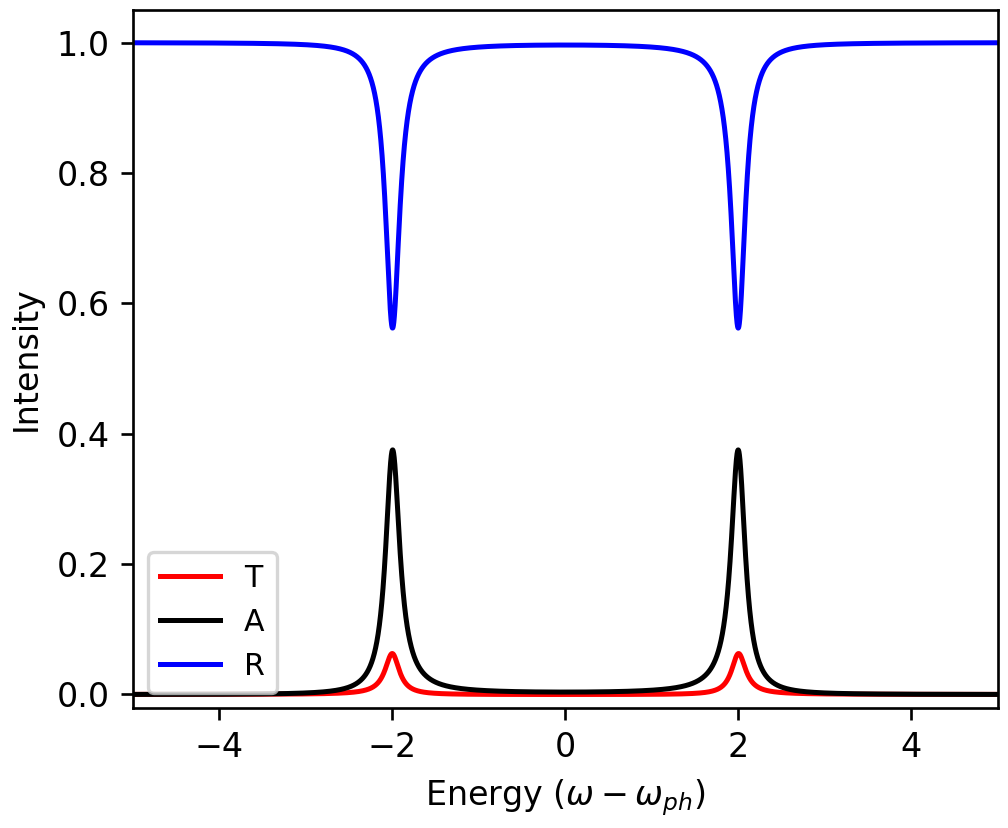
\includegraphics[height=0.41\textheight,keepaspectratio]
          {../figures/linear/fig3a_reproduction.png}\par}
      {\centering\tiny\color{gray}JCP Fig.~3(a)\par}
    \end{column}
    \begin{column}{0.48\textwidth}
      {\centering
        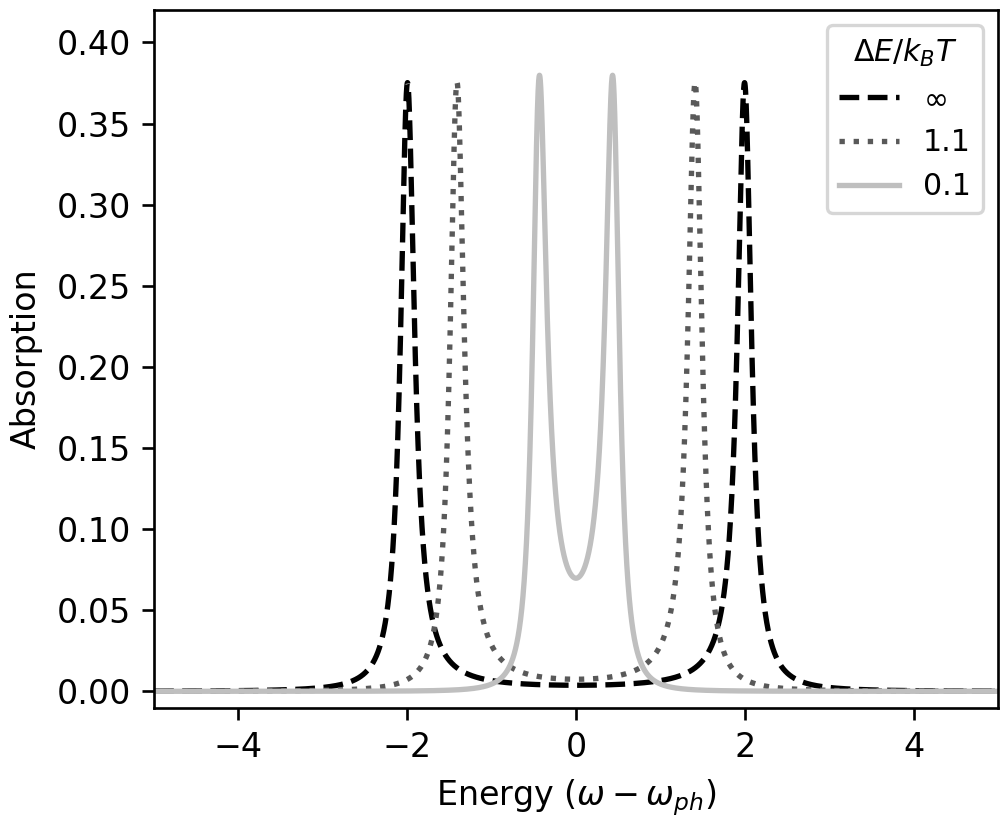
\includegraphics[height=0.41\textheight,keepaspectratio]
          {../figures/linear/fig3b_reproduction.png}\par}
      {\centering\tiny\color{gray}JCP Fig.~3(b)\par}
    \end{column}
  \end{columns}

  \vspace{0.3em}

  \begin{columns}[c,onlytextwidth]
    \begin{column}{0.48\textwidth}
      {\centering
        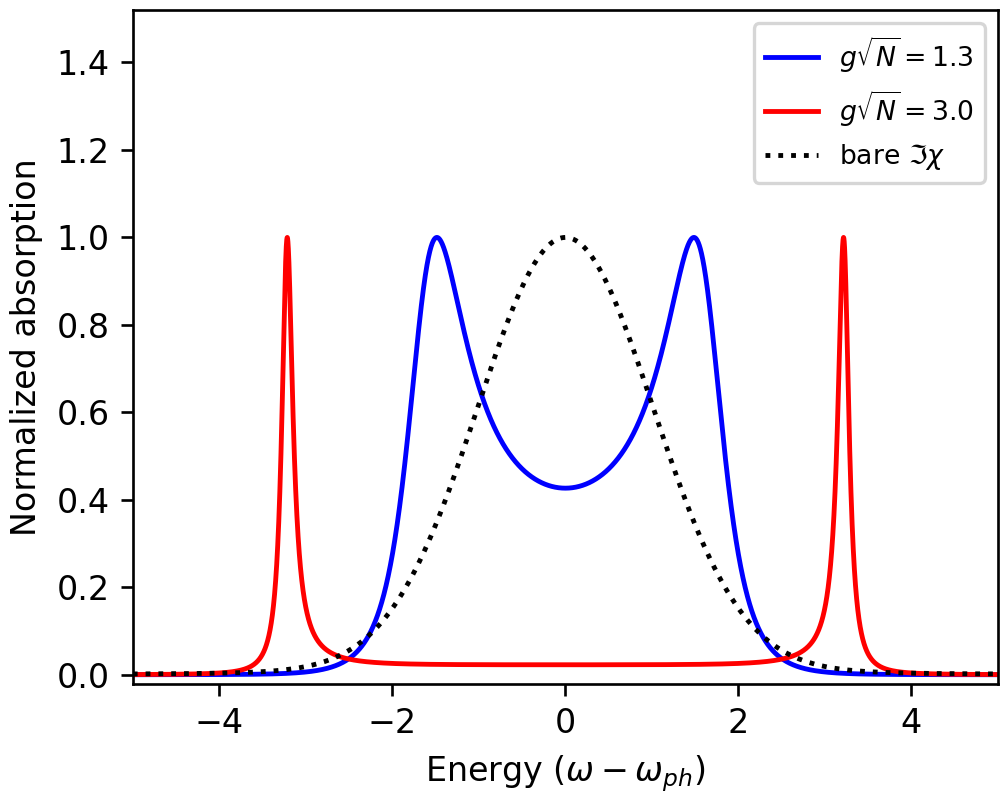
\includegraphics[height=0.41\textheight,keepaspectratio]
          {../figures/linear/fig4c_reproduction.png}\par}
      {\centering\tiny\color{gray}JCP Fig.~4(c)\par}
    \end{column}
    \begin{column}{0.48\textwidth}
      {\centering
        
\includegraphics[height=0.41\textheight,keepaspectratio]
          {../figures/nonlinear/fig3_reproduction.png}\par}
      {\centering\tiny\color{gray}PRL Fig.~3\par}
    \end{column}
  \end{columns}

  \vspace{0.25em}

  {\centering\tiny\color{gray}
    Codex（GPT-5.6 Sol）一次完整复现工作流运行约 47 min，
    已有复现结果与原文基本一致。\par}

\end{frame}

\backmatter

\begin{frame}{二能级分子线性极化率}

  \small
  \setlength{\abovedisplayskip}{3pt}
  \setlength{\belowdisplayskip}{3pt}

  {\footnotesize\textbf{1. 一阶光学相干运动方程}}
  \[
    \dot\rho_{eg}^{(1)}
    =-\left(\ii\omega_0+\frac{\gamma}{2}\right)\rho_{eg}^{(1)}
    +\ii\frac{\mu_{eg}}{\hbar}(p_g-p_e)E(t).
  \]

  \vspace{0.4em}
  {\footnotesize\textbf{2. 单频驱动下的频域解}}
  \[
    \rho_{eg}^{(1)}(\omega)
    =-\frac{\mu_{eg}}{\hbar}
    \frac{p_g-p_e}{\omega-\omega_0+\ii\gamma/2}E(\omega).
  \]

  \vspace{0.4em}
  {\footnotesize\textbf{3. 第一篇腔耦合归一化后的极化率}}
  \vspace{1.5em}
  \[
    \chi_{\mathrm{2LS}}(\omega)
    =-\frac{
      \physmark{Plum}{p26G2}{G^2}
      \physmark{Bittersweet}{p26pgpe}{(p_g-p_e)}
    }{\omega-\physmark{NavyBlue}{p26w0}{\omega_0}
      +\ii\physmark{OliveGreen}{p26gam}{\gamma/2}}
  \]
  \begin{tikzpicture}[overlay,remember picture,>=stealth,
      nodes={align=center,inner ysep=1pt},<-]
    \path (p26G2.south) ++ (-0.9,3.8em)
      node[anchor=north,color=Plum!85] (p26G2text)
      {\textsf{\footnotesize 集体耦合权重}};
    \draw[color=Plum] (p26G2.north) |- (p26G2text.south);
    \path (p26pgpe.south) ++ (1.2,3.8em)
      node[anchor=north,color=Bittersweet!85] (p26pgpetext)
      {\textsf{\footnotesize 布居差 / 净响应权重}};
    \draw[color=Bittersweet] (p26pgpe.north) |- (p26pgpetext.south);
    \path (p26w0.south) ++ (-0.75,-0.8em)
      node[anchor=north,color=NavyBlue!85] (p26w0text)
      {\textsf{\footnotesize 共振位置}};
    \draw[color=NavyBlue] (p26w0.south) |- (p26w0text.north);
    \path (p26gam.south) ++ (1.5,-2.0em)
      node[anchor=north,color=OliveGreen!85] (p26gamtext)
      {\textsf{\footnotesize 光学相干线宽}};
    \draw[color=OliveGreen] (p26gam.south) |- (p26gamtext.north);
  \end{tikzpicture}
  \vspace{2.2em}

\end{frame}

\begin{frame}{标准腔输入--输出关系}

  \footnotesize
  \setlength{\abovedisplayskip}{2pt}
  \setlength{\belowdisplayskip}{2pt}

  \begin{columns}[c,onlytextwidth]
    \begin{column}{0.30\textwidth}
      {\centering
        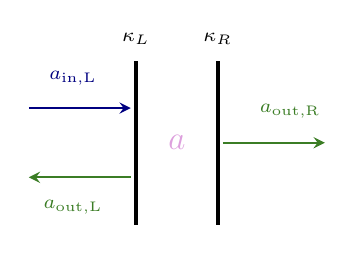
\begin{tikzpicture}[>=stealth,x=0.8cm,y=0.8cm,
            every node/.style={inner sep=2pt,font=\scriptsize}]
          \draw[line width=1.3pt] (1.1,-1.3) -- (1.1,1.3);
          \draw[line width=1.3pt] (2.4,-1.3) -- (2.4,1.3);
          \node at (1.1,1.65) {$\kappa_L$};
          \node at (2.4,1.65) {$\kappa_R$};
          \node[text=Plum,font=\large] at (1.75,0) {$a$};
          \draw[->,NavyBlue,thick] (-0.6,0.55) -- (1.02,0.55);
          \node[text=NavyBlue] at (0.1,1.02) {$a_{\mathrm{in,L}}$};
          \draw[->,OliveGreen,thick] (1.02,-0.55) -- (-0.6,-0.55);
          \node[text=OliveGreen] at (0.1,-1.02) {$a_{\mathrm{out,L}}$};
          \draw[->,OliveGreen,thick] (2.48,0) -- (4.1,0);
          \node[text=OliveGreen] at (3.55,0.5) {$a_{\mathrm{out,R}}$};
        \end{tikzpicture}\par}
      {\centering $\kappa=\kappa_L+\kappa_R$。\par}
      \vspace{0.5em}
      {\fontsize{7}{8.5}\selectfont\color{gray}
        相干振幅；$a_{\mathrm{in,R}}=0$。\par
        $\omega_c\equiv\omega_{\mathrm{ph}}$（p\pageref{frame:cavity-response}）。\par
        单频 $e^{-\ii\omega t}$；旋波、马尔可夫近似。
      }
    \end{column}
    \begin{column}{0.67\textwidth}
      \[
        \dot a=-\left(\ii\omega_c+\tfrac\kappa2\right)a
          +\sqrt{\kappa_L}\,a_{\mathrm{in,L}}+\mathcal F_{\mathrm{mol}}.
      \]
      {\scriptsize\color{gray}
        线性分子反馈：$\mathcal F_{\mathrm{mol}}(\omega)=\ii\chi(\omega)a(\omega)$。
      }
      \[
        \begin{aligned}
          a(\omega)&=\ii\sqrt{\kappa_L}\,D^R(\omega)a_{\mathrm{in,L}}(\omega),\\
          D^R(\omega)&=\frac{1}{\omega-\omega_c+\ii\kappa/2+\chi(\omega)}.
        \end{aligned}
      \]
      \[
        a_{\mathrm{out,L}}=a_{\mathrm{in,L}}-\sqrt{\kappa_L}\,a,
        \qquad a_{\mathrm{out,R}}=-\sqrt{\kappa_R}\,a.
      \]
      {\scriptsize
        振幅比：$r=a_{\mathrm{out,L}}/a_{\mathrm{in,L}}$，
        $t=a_{\mathrm{out,R}}/a_{\mathrm{in,L}}$。
      }
      \[
        r(\omega)=1-\ii\kappa_LD^R(\omega),
        \qquad t(\omega)=-\ii\sqrt{\kappa_L\kappa_R}\,D^R(\omega).
      \]
      \[
        T=|t|^2,\qquad R=|r|^2,\qquad A=1-T-R.
      \]
    \end{column}
  \end{columns}

  \vspace{0.4em}
  \[
    T(\omega)=\frac{\kappa_L\kappa_R}
      {|\omega-\omega_c+\ii\kappa/2+\chi(\omega)|^2},
    \qquad
    A(\omega)=\frac{2\kappa_L\operatorname{Im}\chi(\omega)}
      {|\omega-\omega_c+\ii\kappa/2+\chi(\omega)|^2}.
  \]

  {\fontsize{6.3}{7.4}\selectfont\color{gray}
    PRL 保留自身输入归一化；本页端口场取相反整体相位，
    $\sqrt{\kappa_L}a_{\mathrm{in,L}}=-\eta f(t)e^{-\ii\omega_l t}$。
  }
  \papersource{JCP 160, 154107 (2024), Eqs.~(27), (32)--(34), (A9), (A13), (B9); PRL SM S2.}

\end{frame}


\end{document}
